% !TEX spellcheck = en-US
\chapter{Probabilistic Models}
\label{cha:models} 
Pose estimation is about estimating the position and orientation of the body frame~$b$ in the navigation frame $n$. This problem is illustrated in \Figureref{fig:models-poseEstimation}, where the position and orientation of the body changes from time $t_1$ to time $t_2$. In this chapter, we will introduce the concept of probabilistic models and discuss different modeling choices when using inertial sensors for pose estimation. 

The subject of probabilistic modeling is introduced in \Sectionref{sec:models-probModeling}. Most complexity in pose estimation lies in the nonlinear nature of the orientation and the fact that orientation can be parametrized in different ways. How to parametrize the orientation is therefore a crucial modeling choice in any pose estimation algorithm. Because of this, we will discuss different parametrizations for the orientation in \Sectionref{sec:models-paramOri} and in \Sectionref{sec:models-probModelingOri} we will discuss how these different parametrizations can be used in probabilistic modeling. 

Our probabilistic models consist of three main components. First, in \Sectionref{sec:models-measModels}, we introduce models describing the knowledge about the pose that can be inferred from the measurements. Second, in \Sectionref{sec:models-stateDynamics}, we model how the sensor pose changes over time. Finally, in \Sectionref{sec:models-prior}, models of the initial pose are introduced. 

The chapter will conclude with a discussion on the resulting probabilistic models in \Sectionref{sec:models-resultingProbModel}. The models that will be used in the position and orientation estimation algorithms in \Chapterref{cha:orientationEstimation} will be introduced in this section.

\begin{figure}
  	\centering
    	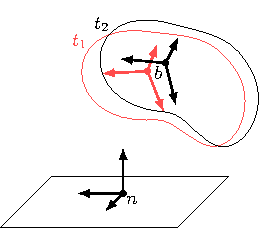
\includegraphics[scale = 1]{figure3_1.pdf}
    	\caption{An illustration of the pose estimation problem. We want to express the position and orientation of the moving body frame $b$ at times $t_1$ and $t_2$ with respect to the navigation frame $n$.}
    	\label{fig:models-poseEstimation}
\end{figure}

\section{Introduction}
\label{sec:models-probModeling}
Probabilistic models constitute the foundation of the estimation algorithms in \Chapterref{cha:orientationEstimation}. In this section we will introduce the concept of probabilistic modeling and the notation that is used in building our models. Models are used to describe the information about the \emph{dynamics} and the available \emph{measurements}. These models are subsequently used in combination with the measurements to \emph{infer} some knowledge. The knowledge that we are interested in is the pose of the sensor and we use information about the \emph{sensor dynamics} and the available measurements (amongst others, inertial measurements). A simplified case where probabilistic modeling is used to estimate the position of a sensor is given in \Exampleref{ex:models-probModeling}.

\begin{myexample}{Probabilistic modeling}%
\label{ex:models-probModeling}%
Let us estimate the 2D position $p_t$ of a sensor at time $t$ from two position measurements
\begin{align*}
y_t^1 = \begin{pmatrix} 0 & 0 \end{pmatrix}^\Transp, \qquad y_t^2 = \begin{pmatrix} 2 & 0 \end{pmatrix}^\Transp.
\end{align*}
A straightforward suggestion for an estimate of the position would be $\hat{p}_t = \begin{pmatrix} 1 & 0 \end{pmatrix}^\Transp$. Let us now assume that we know the accuracy of the sensors and represent this in terms of the following probabilistic models 
\begin{align*}
y_t^1 &= p_t + e_t^1, &e_t^1 &\sim \mathcal{N}( 0, 0.25 \, \mathcal{I}_2 ), \\
y_t^2 &= p_t + e_t^2, &e_t^2 &\sim \mathcal{N}( 0,\mathcal{I}_2 ),
\end{align*}
where $\mathcal{I}_2$ denotes a $2 \times 2$ identity matrix. A reasonable position estimate would instead be
\begin{align*}
p_t \sim \mathcal{N} \left( \begin{pmatrix} 0.4 \\ 0 \end{pmatrix}, 0.2 \, \mathcal{I}_2 \right) .
\end{align*}
We will not go into details about how this estimate is derived. Instead, we would like to point out two differences between this position estimate and our initial suggestion $\hat{p}_t$. First, based on the knowledge of the accuracy of the sensors, it is sensible to trust the measurement from the first sensor more than the measurement from the second sensor. Our improved position estimate is therefore closer to the measurement of the first sensor than our initial suggestion $\hat{p}_t$. Furthermore, based on the accuracy of the sensors, it is possible to derive the accuracy of our estimate. 

Now consider the case where we are also interested in estimating the position $p_{t+1}$. Knowledge that the sensor is worn by a human or placed in a car, would give us information about how far the sensor can travel from time $t$ to time $t+1$. If the sensor would be placed in for instance a train, the motion would even be constrained to be along the tracks. Incorporating this information about the dynamics of the sensor will improve the estimate of $p_{t+1}$.
\end{myexample}

We split the knowledge that we want to infer into the unknown \emph{time-varying states} $x_t$ for $t = 1, \hdots, N$, or equivalently $x_{1:N}$, and the unknown \emph{constant parameters} $\theta$. We denote the measurements by $y_k$ for $k = 1, \hdots, K$. The times $k$ at which these measurements are obtained do not necessarily correspond with the times $t$ at which the states are defined. It is also not necessary for all sensors to sample at the same frequency. As discussed in \Sectionref{sec:sensors-errors}, the inertial sensors are typically sampled at fairly high rates to capture high-frequency dynamics. In stand-alone, wired \glspl{imu}, all sensors typically have the same, constant sampling frequency. Specifically in the case of wireless sensors and smartphones, however, the sampling frequencies can vary both over sensors and over time. In the remainder, we assume that the times $t$ at which the states are defined coincide with the times $k$ at which the gyroscopes sample. Hence, we denote the gyroscope measurements $y_{\omega,t}$ with $t = 1, \hdots N$. For notational convenience, we will also use the subscript~$t$ for the measurements from other sensors. Note that these are not required to actually sample at each time $t$ for $t = 1, \hdots N$. For instance, magnetometers in smartphones often sample either at equal or at half the sampling frequencies of the inertial sensors, while position aiding sensors like for instance \gls{gnss} or \gls{uwb} typically sample at much lower sampling frequencies. 

Our aim is now to infer information about the states $x_{1:N}$ and the parameters $\theta$ using the measurements $y_{1:N}$ and the probabilistic models. This can be expressed in terms of a \emph{conditional probability distribution}
\begin{align}
\label{eq:models-smoothing}
p(x_{1:N}, \theta \mid y_{1:N} ),
\end{align}
where $p ( a \mid b )$ denotes the conditional probability of $a$ given $b$. In the pose estimation problem, we are interested in obtaining \emph{point estimates} which we denote $\hat{x}_{1:N}$ and $\hat{\theta}$. It is typically also highly relevant to know how \emph{certain} we are about these estimates. This is often expressed in terms of a \emph{covariance}. When the distribution~\eqref{eq:models-smoothing} is Gaussian, the distribution is completely described in terms of its mean 
and covariance. 

In~\eqref{eq:models-smoothing} we assume that all measurements $y_{1:N}$ are used to obtain the posterior distribution of $x_{1:N}$ and $\theta$. This is referred to as \emph{smoothing}. Although it makes sense to use all available information to obtain the best estimates, a downside of smoothing is that we need to wait until all measurements are collected before the pose can be computed. Because of this, in many applications, we are also interested in \emph{filtering}. In filtering we estimate $x_t$ using all measurements up to and including time $t$. One way of dealing with constant parameters in filtering is to treat them as slowly time-varying. In this case, they can be considered to be included in the time-varying states $x_t$. The filtering problem can be expressed in terms of the conditional probability distribution
\begin{align}
\label{eq:models-filtering}
p(x_t \mid y_{1:t} ).
\end{align}
We have now introduced smoothing, where the states $x_{1:N}$ are estimated simultaneously, and filtering, where at each time instance the state $x_t$ is estimated. There is a large range of intermediate methods, where a batch of states $x_{t - L_1 : t + L_2}$, with $L_1$ and $L_2$ being positive integers, is estimated using the measurements $y_{1:t}$. This is related to fixed-lag smoothing and moving horizon estimation \citep{johansen:2011,raoRL:2001}.

\begin{figure}
  	\centering
    	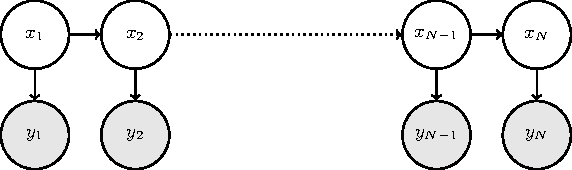
\includegraphics[scale = 1]{figure3_2.pdf}
    	\caption{An illustration of the structure of the pose estimation problem.}
    	\label{fig:models-structureProblem}
\end{figure}

The topic of how to estimate the conditional probability distributions for position and orientation estimation will be introduced in \Chapterref{cha:orientationEstimation}. We will now instead take a closer look at these distributions and their different components. A fundamental assumption here is that we assume that our models possess the \emph{Markov property}, implying that all information up to the current time $t$ is contained in the state $x_t$. This is illustrated in \Figureref{fig:models-structureProblem} in terms of a \emph{probabilistic graphical model}~\citep{bishop:2006}. The state $x_{t+1}$ can be seen to depend on $x_t$ and to result in the measurements $y_{t+1}$. It is conditionally independent of $x_{1:t-1}$ given the state~$x_t$. Using Bayes' rule and the Markov property, the conditional distributions~\eqref{eq:models-smoothing} and~\eqref{eq:models-filtering} can be decomposed as
\begin{subequations}
\label{eq:models-smoothingFiltProbs}
\begin{align}
\hspace{-2mm} p(x_{1:N}, \theta \mid y_{1:N} ) &\propto p(\theta) p(x_1 \mid \theta) \prod_{t=2}^N p(x_t \mid x_{t-1}, \theta) \prod_{t=1}^N p(y_t \mid x_t, \theta) \label{eq:models-smoothingProbs}, \hspace{-1mm} \\
p(x_t \mid y_{1:t} ) &\propto p(y_t \mid x_t) p(x_t \mid y_{1:t-1}) \label{eq:models-filteringProbs}.
\end{align}
\end{subequations}
The predictive distribution $p(x_t \mid y_{1:t-1})$ can be computed by \emph{marginalizing out} the previous state $x_{t-1}$ as
\begin{align}
&p(x_t \mid y_{1:t-1}) = \int p(x_t \mid x_{t-1}) p(x_{t-1} \mid y_{1:t-1}) \, \dint x_{t-1}.
\end{align}
In~\eqref{eq:models-smoothingFiltProbs}, $p(\theta)$ and $p(x_1 \mid \theta)$ encode our \emph{prior} information of $\theta$ and the knowledge of the state $x_1$ given $\theta$, respectively. The \emph{dynamics} are modeled in terms of $p(x_{t+1} \mid x_{t} , \theta)$ and $p(x_{t+1} \mid x_{t})$. The distributions $p(y_t \mid x_{t} , \theta)$ and $p(y_t \mid x_{t})$ model the information given by the measurements about the state and the parameters.

The dynamics of the state can be modeled in terms of a nonlinear function $f_t(\cdot)$ as
\begin{align}
\label{eq:models-dynamics}
x_{t+1} = f_t (x_t, w_t).
\end{align}
The uncertainty of the dynamic model is modeled in terms of $w_t$, which is often referred to as the \emph{process noise}. The model~\eqref{eq:models-dynamics} provides information about the distribution $p(x_{t+1} \mid x_t)$. More explicitly, if $w_t$ is Gaussian additive noise with $w_t \sim \mathcal{N}(0,Q)$, then
\begin{align}
p(x_{t+1} \mid x_t) \sim \mathcal{N}(x_{t+1} \, ; \, f_t(x_t), Q),
\end{align}
where we use the notation $\mathcal{N}(x_{t+1} \, ; \, f_t(x_t), Q)$ to explain that the random variable $x_{t+1}$ is normal distributed with mean $f_t(x_t)$ and covariance $Q$. 

The information given by the measurements about the state $x_t$ can be modeled as
\begin{align}
\label{eq:models-measEqn}
y_{t} = h_t (x_t, e_t),
\end{align}
where $h_t(\cdot)$ is a possibly nonlinear function and $e_t$ is the measurement noise. The measurement model~\eqref{eq:models-measEqn} provides information about the distribution $p(y_t \mid x_t)$. The combination of~\eqref{eq:models-dynamics},~\eqref{eq:models-measEqn} and a model of the prior $p(x_1)$ is referred to as a \emph{state space model} \citep{kailath:1980} which is widely used in a large number of fields.

\section{Parametrizing orientation}
\label{sec:models-paramOri}
Rotating a vector in $\mathbb{R}^3$ changes the \emph{direction} of the vector while retaining its \emph{length}. The group of rotations in $\mathbb{R}^3$ is the special orthogonal group $\SO{3}$. In this section we introduce four different ways of parametrizing orientations. Note that these describe the same quantity and can hence be used interchangeably. The different parametrizations can be converted to one another, see also \Appendixref{app:rotation}. There are differences in for instance the number of parameters used in the representation, the singularities and the uniqueness. 

\subsection{Rotation matrices}
We encountered rotation matrices already in \Chapterref{cha:sensors}. Rotation matrices $R \in \mathbb{R}^{3\times3}$ have the following properties
\begin{align}
  \label{eq:models-rotMatrixProperties}
  R R^\Transp = R^\Transp R = \mathcal{I}_3, \qquad \det R = 1.
\end{align}
The properties~\eqref{eq:models-rotMatrixProperties} provide an interpretation of the name special orthogonal group $\SO{3}$. All orthogonal matrices of dimension $3 \times 3$ have the property $R R^\Transp = R^\Transp R = \mathcal{I}_3$ and are part of the orthogonal group $O(3)$. The notion \emph{special} in $\SO{3}$ specifies that only matrices with $\det R = 1$ are considered rotations.

Consider two coordinate frames denoted $u$ and $v$. As was illustrated in \Exampleref{ex:sensors-rotationVectors}, a vector $x$ expressed in the $v$-frame can be rotated to the $u$-frame as
\begin{subequations}
\begin{align}
\label{eq:models-rotxVtoU}
x^\text{u} &= R^\text{uv} x^\text{v}, \\
\intertext{and conversely we have}
  \label{eq:models-rotxUtoV}
  x^\text{v} &= \left( R^\text{uv} \right)^\Transp x^\text{u} = R^\text{vu} x^\text{u}.
\end{align}
\end{subequations}
A rotation matrix is a unique description of the orientation. It has $9$ components which depend on each other as defined in~\eqref{eq:models-rotMatrixProperties}.

\subsection{Rotation vector}
As described by Leonhard Euler in \cite{euler:1775}, a rotation around a point is always equivalent to a single rotation around some axis through this point, see \cite{palaisPR:2009} for a number of proofs. This is generally referred to as \emph{Euler's rotation theorem}. Hence, it is possible to express the rotation between two coordinate frames in terms of an angle $\alpha$ and a unit vector $n$ around which the rotation takes place. In this section, we will derive a relation between the representation $\alpha, n$ and the rotation matrix parametrization from the previous section. Instead of directly considering the rotation of a coordinate frame, we start by considering the rotation of a vector. Note that a counterclockwise rotation of the coordinate frame is equivalent to a clockwise rotation of a vector, see \Exampleref{ex:models-rotVectorCoordFrame}.

\begin{myexample}{Rotation of a coordinate frame and rotation of a vector}%
\label{ex:models-rotVectorCoordFrame}%
Consider the 2D example in \Figureref{fig:models-rotateVectorCoordFrame}, where on the left, a vector $x$ is rotated clockwise by an angle $\alpha$ to $x_\star$. This is equivalent to (on the right) rotating the coordinate frame $v$ counterclockwise by an angle $\alpha$. Note that $x^\text{v}_\star = x^\text{u}$.

\begin{figure}
      \centering
      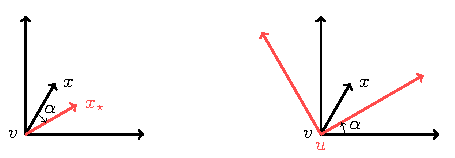
\includegraphics[scale = 1]{figure3_3.pdf}
      \caption[]{Left: clockwise rotation $\alpha$ of the vector $x$ to the vector $x_\star$. Right: counterclockwise rotation $\alpha$ of the coordinate frame $v$ to the coordinate frame~$u$.}
      \label{fig:models-rotateVectorCoordFrame}
\end{figure}
\end{myexample}

In \Figureref{fig:models-axisAngle}, a vector $x$ is rotated an angle $\alpha$ around the unit vector~$n$. We denote the rotated vector by $x_\star$. Suppose that $x$ as expressed in the coordinate frame $v$ is known (and denoted $x^\text{v}$) and that we want to express $x_\star^\text{v}$ in terms of $x^\text{v}$, $\alpha$ and $n$. It can first be recognized that the vector $x$ can be decomposed into a component parallel to the axis $n$, denoted $x_\parallel$, and a component orthogonal to it, denoted $x_\perp$, as
\begin{subequations}
\begin{align}
x^\text{v} &= x^\text{v}_\parallel + x^\text{v}_\perp. \\
\intertext{Based on geometric reasoning we can conclude that}
x^\text{v}_\parallel &= \left( x^\text{v} \cdot n^\text{v} \right) n^\text{v},
\end{align} 
\end{subequations} 
where $\cdot$ denotes the inner product. Similarly, $x_\star^\text{v}$ can be decomposed as
\begin{subequations}
\begin{align}
x^\text{v}_\star &= \left( x^\text{v}_\star \right)_\parallel + \left( x^\text{v}_\star \right)_\perp,
\intertext{where}
\left( x^\text{v}_\star \right)_\parallel &= x^\text{v}_\parallel, \\
\left( x^\text{v}_\star \right)_\perp &= x^\text{v}_\perp \cos \alpha + \left( x^\text{v} \times n^\text{v} \right) \sin \alpha.
\end{align}
\end{subequations}
Hence, $x^\text{v}_\star$ can be expressed in terms of $x^\text{v}$ as
\begin{align}
  x_\star^\text{v} 
  &= (x^\text{v} \cdot n^\text{v}) n^\text{v} 
    + (x^\text{v} - (x^\text{v} \cdot n^\text{v}) n^\text{v})\cos\alpha
    + (x^\text{v} \times n^\text{v})\sin\alpha \nonumber \\
  &= x^\text{v} \cos\alpha 
    + n^\text{v} (x^\text{v} \cdot n^\text{v})(1-\cos\alpha)
    - (n^\text{v} \times x^\text{v})\sin\alpha.
\end{align}
Denoting the rotated coordinate frame the $u$-frame and using the equivalence between $x^\text{v}_\star$ and $x^\text{u}$ as shown in \Exampleref{ex:models-rotVectorCoordFrame}, this implies that 
\begin{align}
  \label{eq:kin-rotation-aa}
  x^\text{u} = x^\text{v} \cos\alpha 
    + n^\text{v} (x^\text{v} \cdot n^\text{v})(1-\cos\alpha)
    - (n^\text{v} \times x^\text{v})\sin\alpha.
\end{align}
This equation is commonly referred to as the \emph{rotation formula} or \emph{Euler's formula}
\citep{shuster:1993}. Note that the combination of $n$ and
$\alpha$, or $\oriError = n \alpha$, is denoted as the \emph{rotation vector}
or the \emph{axis-angle parameterization}.  

\begin{figure}
      \centering
      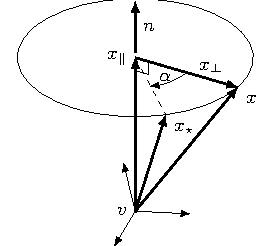
\includegraphics[scale = 1]{figure3_4.pdf}
      \caption[]{Clockwise rotation of a vector $x$ by an angle $\alpha$
        around the unit vector~$n$. The rotated vector is denoted by $x_\star$. The vector $x$ is decomposed in a component $x_\parallel$ that is parallel to the axis $n$, and a component $x_\perp$ that is orthogonal to it.}
      \label{fig:models-axisAngle}
\end{figure}

To show the equivalence between~\eqref{eq:kin-rotation-aa} and the rotation matrix parametrization, we will rewrite~\eqref{eq:kin-rotation-aa}. Here, we make use of the fact that a cross product can be written as a matrix vector product. Given vectors $u$ and $v$ we have, 
\begin{align}
  \label{eq:models-crossproductMatrix}
  u \times v &= [u \times] v = - [v \times] u, 
  \qquad 
  [u \times] \triangleq 
  \begin{pmatrix}
    0 & -u_3 & u_2 \\
    u_3 & 0 & -u_1 \\
    -u_2 & u_1 & 0 
  \end{pmatrix},
\end{align}
where $u_1, u_2, u_3$ denote the three components of the vector $u$. Furthermore, given vectors $u$, $v$ and $w$, multiple cross products can be expanded in terms of the inner product as
\begin{align}
  \label{eq:models-crossproductExp}
  u \times (v \times w)
    = v (w \cdot u) - w (u \cdot v).
\end{align}
Using these relations, \eqref{eq:kin-rotation-aa} can be rewritten as
\begin{align}
  x^\text{u} &= x^\text{v} \cos\alpha 
    + n^\text{v} (x^\text{v} \cdot n^\text{v})(1-\cos\alpha)
    - (n^\text{v} \times x^\text{v})\sin\alpha \nonumber\\
    &= x^\text{v} \cos\alpha 
     + (n^\text{v} \times (n^\text{v} \times x^\text{v}) 
       + x^\text{v})(1-\cos\alpha)
     - (n^\text{v} \times x^\text{v})\sin\alpha \nonumber \\
  \label{eq:models-axisAngle-rotMatrix-der}
  &= \left( \mathcal{I}_3 - \sin\alpha [n^\text{v} \times] 
        + (1-\cos\alpha)[n^\text{v} \times]^2
      \right) x^\text{v}.
\end{align}
Comparing~\eqref{eq:models-axisAngle-rotMatrix-der} and~\eqref{eq:models-rotxVtoU}, it can be seen that a rotation matrix can be parametrized in terms of $\alpha, n$ as
\begin{align}
\label{eq:models-axisAngle-rotMatrix}
R^\text{uv}(n^\text{v},\alpha) = \mathcal{I}_3 - \sin\alpha [n^\text{v} \times] 
        + (1-\cos\alpha)[n^\text{v} \times]^2.
\end{align}
Note that equivalently, $R^\text{uv}(n^\text{v},\alpha)$ can also be written as
\begin{align}
\label{eq:models-rotMatrixAxisAngleExp}
R^\text{uv}(n^\text{v},\alpha) = \exp \left( - \alpha [n^\text{v} \times] \right), 
\end{align}
since 
\begin{align}
\label{eq:models-rotMatrixAxisAngle}
&\exp \left( - \alpha [n^\text{v} \times] \right) = \sum_{k = 0}^\infty \tfrac{1}{k!} \left( - \alpha [n^\text{v} \times] \right)^k \nonumber \\
&\qquad = \mathcal{I}_3 - \alpha [n^\text{v} \times] + \tfrac{1}{2!} \alpha^2 [n^\text{v} \times]^2 + 
\tfrac{1}{3!} \alpha^3 [n^\text{v} \times] - 
\tfrac{1}{4!} \alpha^4 [n^\text{v} \times]^2 - \hdots \nonumber \\
&\qquad= \mathcal{I}_3 - \left( \alpha - \tfrac{1}{3!} \alpha^3 + \hdots \right) [n^\text{v} \times] + 
\left( \tfrac{1}{2!} \alpha^2 - \tfrac{1}{4!} \alpha^4 + \hdots \right) [n^\text{v} \times]^2 \nonumber \\
&\qquad= \mathcal{I}_3 - \sin\alpha [n^\text{v} \times] + (1-\cos\alpha)[n^\text{v} \times]^2.
\end{align}
The rotation vector introduced in this section parametrizes the orientation in only three parameters. It is, however, not a unique parametrization since adding $2 \pi$ to any angle $\alpha$ results in the same orientation. This is called \emph{wrapping}. As shown in~\eqref{eq:models-axisAngle-rotMatrix} and~\eqref{eq:models-rotMatrixAxisAngleExp}, the rotation matrix can straightforwardly be expressed in terms of the axis-angle representation. 

\subsection{Euler angles}
Rotation can also be defined as a consecutive rotation around three axes in terms of so-called \emph{Euler angles}. We use the convention $(z,y,x)$ which first rotates an angle $\psi$ around the $z$-axis, subsequently an angle $\theta$ around the $y$-axis and finally an angle $\phi$ around the $x$-axis. These angles are illustrated in \Figureref{fig:models-eulerAngles}. Assuming that the $v$-frame is rotated by $(\psi, \theta, \phi)$ with respect to the $u$-frame as illustrated in this figure, the rotation matrix $R^\text{uv}$ is given by 

{\footnotesize{
\begin{align}
\label{eq:models-rotMatrix}
R^\text{uv} &= R^\text{uv}(e_1, \phi) R^\text{uv}(e_2, \theta) R^\text{uv}(e_3, \psi) \\
&= \begin{pmatrix} 1 & 0 & 0 \\ 0 & \cos \phi & \sin \phi \\ 0 & -\sin \phi & \cos \phi \end{pmatrix}
\begin{pmatrix} \cos \theta & 0 & -\sin \theta \\ 0 & 1 & 0 \\ \sin \theta & 0 & \cos \theta \end{pmatrix}
\begin{pmatrix} \cos \psi & \sin \psi & 0 \\ -\sin \psi & \cos \psi & 0 \\ 0 & 0 & 1 \end{pmatrix} \nonumber \\
&= \begin{pmatrix} \cos \theta \cos \psi & \cos \theta \sin \psi & -\sin \theta \\ 
\sin \phi \sin \theta \cos \psi - \cos \phi \sin \psi & \sin \phi \sin \theta \sin \psi + \cos \phi \cos \psi & \sin \phi \cos \theta \\ 
\cos \phi \sin \theta \cos \psi + \sin \phi \sin \psi & \cos \phi \sin \theta \sin \psi - \sin \phi \cos \psi & \cos \phi \cos \theta \end{pmatrix},\nonumber
\end{align}}}%
where we make use of the notation introduced in~\eqref{eq:models-axisAngle-rotMatrix} and the following definition of the unit vectors 
\begin{align}
e_1 = \begin{pmatrix} 1 & 0 & 0 \end{pmatrix}^\Transp, \quad e_2 = \begin{pmatrix} 0 & 1 & 0 \end{pmatrix}^\Transp, \quad e_3 = \begin{pmatrix} 0 & 0 & 1 \end{pmatrix}^\Transp.
\end{align}
The $\psi, \theta, \phi$ angles are also often referred to as yaw (or heading), pitch and roll, respectively. Furthermore, roll and pitch together are often referred to as inclination. 

Similar to the rotation vector, Euler angles parametrize orientation as a three-dimensional vector. Euler angle representations are not unique descriptions of a rotation for two reasons. First, due to wrapping of the Euler angles, the rotation $(0, 0, 0)$ is for instance equal to $(0, 0, 2 \pi k)$ for any integer $k$.  Furthermore, setting $\theta = \tfrac{\pi}{2}$ in~\eqref{eq:models-rotMatrix}, leads to
\begin{align}
R^\text{uv} &= \begin{pmatrix} 0 & 0 & -1 \\ 
\sin \phi \cos \psi - \cos \phi \sin \psi & \sin \phi \sin \psi + \cos \phi \cos \psi & 0 \\ 
\cos \phi \cos \psi + \sin \phi \sin \psi & \cos \phi \sin \psi - \sin \phi \cos \psi & 0 \end{pmatrix} \nonumber \\
&= \begin{pmatrix} 0 & 0 & -1 \\ 
\sin (\phi - \psi) & \cos (\phi - \psi) & 0 \\ 
\cos (\phi - \psi) & - \sin (\phi - \psi) & 0 \end{pmatrix}.
\end{align}
Hence, only the rotation $\phi - \psi$ can be observed. Because of this, for example the rotations $(\tfrac{\pi}{2}, \tfrac{\pi}{2}, 0)$, $(0, \tfrac{\pi}{2}, -\tfrac{\pi}{2})$, $(\pi, \tfrac{\pi}{2},\tfrac{\pi}{2})$ are all three equivalent. This is called \emph{gimbal lock}~\citep{diebel:2006}. 

\begin{figure}
	\centering
	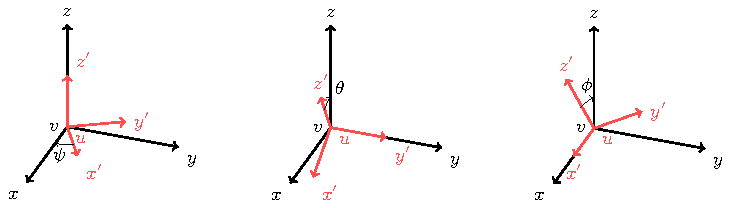
\includegraphics[scale = 1]{figure3_5.pdf}
		\caption{Definition of Euler angles as used in this work with left: rotation~$\psi$ around the $z$-axis, middle: rotation~$\theta$ around the $y$-axis and right: rotation~$\phi$ around the $x$-axis.}
	\label{fig:models-eulerAngles}
\end{figure}

\subsection{Unit quaternions}
A commonly used parametrization of orientation is that of unit quaternions. Quaternions were first introduced by~\cite{hamilton:1844} and are widely used in orientation estimation algorithms, see \eg \cite{kuipers:1999,hol:2011}. A unit quaternion use a $4$-dimensional representation of the orientation according to
\begin{align}
q = \begin{pmatrix} q_0 & q_1 & q_2 & q_3 \end{pmatrix}^\Transp = \begin{pmatrix} q_0 \\ q_v \end{pmatrix}, \qquad q \in \mathbb{R}^4, \qquad \| q\|_2 = 1.
\end{align}
A unit quaternion is not a unique description of an orientation. The reason for this is that if $q$ represents a certain orientation, then $-q$ describes the same orientation. 

A rotation can be defined using unit quaternions as
\begin{align}
  \label{eq:models-rotatex_q}
  \bar x^\text{u} = 
    q^\text{uv} \odot \bar x^\text{v} \odot \left( q^\text{uv} \right)^\conj,
\end{align}
where $\left( q^\text{uv} \right)^\conj = q^\text{vu}$ denotes the quaternion conjugate, defined as
\begin{align}
\label{eq:models-quatConj}
q^\conj = \begin{pmatrix} q_0 & -q_v^\Transp \end{pmatrix}^\Transp,
\end{align}
and $\bar x^\text{v}$ denotes the quaternion representation of $x^\text{v}$ as 
\begin{align}
\label{eq:models-quatVector}
\bar x^\text{v} = \begin{pmatrix} 0 & (x^\text{v})^\Transp \end{pmatrix}^\Transp.
\end{align}
Note that~\eqref{eq:models-quatVector} is typically not a unit quaternion. The notation $\odot$ denotes the quaternion multiplication given by 
\begin{align}
\label{eq:models-quatMult}
p \odot q = \begin{pmatrix} p_0 q_0 - p_v \cdot q_v \\ p_0 q_v + q_0 p_v + p_v \times q_v \end{pmatrix} = p^\leftMult q = q^\rightMult p,
\end{align}
where 
\begin{align}
\label{eq:models-leftRightQuatMult}
p^\leftMult &\triangleq \begin{pmatrix} p_0 & -p_v^\Transp \\ p_v & p_0 \mathcal{I}_3 + [p_v \times] \end{pmatrix}, \qquad q^\rightMult \triangleq \begin{pmatrix} q_0 & -q_v^\Transp \\ q_v & q_0 \mathcal{I}_3 - [q_v \times] \end{pmatrix}.
\end{align}
Using~\eqref{eq:models-quatConj}--\eqref{eq:models-leftRightQuatMult},~\eqref{eq:models-rotatex_q} can be written as
\begin{align}
\label{eq:models-quatRotInterm}
\bar x^\text{u} &= \left( q^\text{uv} \right)^\leftMult \left( q^\text{vu} \right)^\rightMult \bar x^\text{v} \nonumber \\
&= \begin{pmatrix} q_0 & -q_v^\Transp \\ q_v & q_0 \mathcal{I}_3 + [q_v \times] \end{pmatrix} \begin{pmatrix} q_0 & q_v^\Transp \\ -q_v & q_0 \mathcal{I}_3 + [q_v \times] \end{pmatrix} \begin{pmatrix} 0 \\ x^\text{v} \end{pmatrix} \nonumber \\
&= \begin{pmatrix} 1 & 0_{1 \times 3} \\ 0_{3 \times 1} & q_v q_v^\Transp + q_0^2 \mathcal{I}_3 + 2 q_0 [q_v \times] + [q_v \times]^2 \end{pmatrix} \begin{pmatrix} 0 \\ x^\text{v} \end{pmatrix}.
\end{align}
Comparing~\eqref{eq:models-quatRotInterm} to~\eqref{eq:models-axisAngle-rotMatrix}, it can be recognized that if we choose 
\begin{align}
\label{eq:models-axisAngle-quat}
q^\text{uv}(n^\text{v},\alpha) = \begin{pmatrix} \cos \tfrac{\alpha}{2} \\ - n^\text{v} \sin \tfrac{\alpha}{2} \end{pmatrix}, 
\end{align}
the two rotation formulations are equivalent since
\begin{align}
\bar x^\text{u} &= \begin{pmatrix} 1 & 0_{1 \times 3} \\ 0_{3 \times 1} & \mathcal{I}_3 - 2 \cos \tfrac{\alpha}{2} \sin \tfrac{\alpha}{2} [n^\text{v} \times] + 2 \sin^2 \tfrac{\alpha}{2} [n^\text{v} \times]^2 \end{pmatrix} \begin{pmatrix} 0 \\ x^\text{v} \end{pmatrix} \nonumber \\
&= \begin{pmatrix} 1 & 0_{1 \times 3} \\ 0_{3 \times 1} & \mathcal{I}_3 - \sin \alpha [n^\text{v} \times] + \left( 1 - \cos \alpha \right) [n^\text{v} \times]^2 \end{pmatrix} \begin{pmatrix} 0 \\ x^\text{v} \end{pmatrix}.
\end{align}
Here, we made use of standard trigonometric relations and the fact that since $\| n^\text{v} \|_2= 1$, $n^\text{v} \left( n^\text{v} \right)^\Transp = \mathcal{I}_3 + [n^\text{v} \times]^2$. Hence, it can be concluded that $q^\text{uv}$ can be expressed in terms of $\alpha$ and $n^\text{v}$ as in~\eqref{eq:models-axisAngle-quat}.

Equivalently, $q^\text{uv}(n^\text{v},\alpha)$ can also be written as 
\begin{align}
q^\text{uv}(n^\text{v},\alpha) = \exp( - \tfrac{\alpha}{2} \bar n^\text{v} ) = \sum_{k = 0}^\infty \tfrac{1}{k!} \left( - \tfrac{\alpha}{2} \bar n^\text{v} \right)^k,
\end{align}
where 
\begin{subequations}
\begin{align}
\left( \bar n^\text{v} \right)^0 &= \begin{pmatrix} 1 & 0 & 0 & 0 \end{pmatrix}^\Transp, \\
\left( \bar n^\text{v} \right)^1 &= \begin{pmatrix} 0 & \left( n^\text{v} \right)^\Transp \end{pmatrix}^\Transp, \\
\left( \bar n^\text{v} \right)^2 &= \bar n^\text{v} \odot \bar n^\text{v} = \begin{pmatrix} - \| n^\text{v} \|_2^2 & 0_{3 \times 1} \end{pmatrix}^\Transp = \begin{pmatrix} - 1 & 0_{3 \times 1} \end{pmatrix}^\Transp, \\
\left( \bar n^\text{v} \right)^3 &= \begin{pmatrix} 0 & - \left( n^\text{v} \right)^\Transp \end{pmatrix}^\Transp, 
\end{align}
\end{subequations}
This leads to 
\begin{align}
\label{eq:models-quatAxisAngle}
q^\text{uv}(n^\text{v},\alpha) &= \exp( - \tfrac{\alpha}{2} \bar n^\text{v} ) = \sum_{k = 0}^\infty \tfrac{1}{k!} \left( - \tfrac{\alpha}{2} \bar n^\text{v} \right)^k \nonumber \\
&= \begin{pmatrix} 1 - \tfrac{1}{2!} \tfrac{\alpha^2}{4} + \tfrac{1}{4!} \tfrac{\alpha^4}{16} - \hdots \\
- \tfrac{\alpha}{2} n^\text{v} + \tfrac{1}{3!} \tfrac{\alpha^3}{8} n^\text{v} - \tfrac{1}{5!} \tfrac{\alpha^5}{32} n^\text{v} + \hdots
\end{pmatrix} \nonumber \\
&= \begin{pmatrix} \cos \tfrac{\alpha}{2} \\ - n^\text{v} \sin \tfrac{\alpha}{2}
\end{pmatrix}.
\end{align}
Note the similarity to~\eqref{eq:models-rotMatrixAxisAngleExp} and~\eqref{eq:models-rotMatrixAxisAngle}. The reason why both rotation matrices and unit quaternions can be described in terms of an exponential of a rotation vector will be discussed in \Sectionref{sec:models-linearization}.

\section{Probabilistic orientation modeling}
\label{sec:models-probModelingOri}
The four parametrizations of orientation discussed in \Sectionref{sec:models-paramOri} can be used interchangeably. However, the choice of which parametrization to use as states $x_t$ in the filtering and smoothing problems introduced in \Sectionref{sec:models-probModeling} has significant impact on the workings of the algorithm. An important reason for this is that estimation algorithms typically assume that the unknown states and parameters are represented in Euclidean space. For instance, they assume that the subtraction of two orientations gives information about the difference in orientation and that the addition of two orientations is again a valid orientation. For the four parametrizations discussed in \Sectionref{sec:models-paramOri}, this is generally not true. For instance, due to wrapping and gimbal lock, subtraction of Euler angles and rotation vectors can result in large numbers even in cases when the rotations are similar. Also, addition and subtraction of unit quaternions and rotation matrices do not in general result in a valid rotation. The equality constraints on the norm of unit quaternions and on the determinant and the orthogonality of rotation matrices are typically hard to include in the estimation algorithms. In \Sectionref{sec:models-linearization}, we will discuss a method to represent orientation in estimation algorithms that deals with the issues described above. It is frequently used in the algorithms that will be described in \Chapterref{cha:orientationEstimation}. In \Sectionref{sec:models-altProbOriModels}, we will also discuss some alternative methods to parametrize orientation for estimation purposes. 

\subsection{Linearization}
\label{sec:models-linearization}
As mentioned in \Sectionref{sec:models-paramOri}, the group of rotations in three dimensions is the special orthogonal group $\SO{3}$. More specifically, $\SO{3}$ is a so-called \emph{matrix Lie group}. For a discussion on the properties of matrix Lie groups and on the reasons why $\SO{3}$ is indeed such a group we refer the reader to \eg \cite{barfoot:2016}. Since rotations are a matrix Lie group, there exists an \emph{exponential map} from a corresponding Lie algebra. Using this property, it is possible to represent orientations on $\SO{3}$ using unit quaternions or rotation matrices, while orientation deviations are represented using rotation vectors on $\mathbb{R}^3$, see \eg \cite{bloeschEtAl:2016}. Hence, we encode an orientation $q^\text{nb}_t$ in terms of a \emph{linearization point} parametrized either as a unit quaternion $\tilde{q}^\text{nb}_t$ or as a rotation matrix $\tilde{R}^\text{nb}_t$ and an \emph{orientation deviation} using a rotation vector $\oriError_t$. Assuming that the orientation deviation is expressed in the body frame~$n$,\footnote{A similar derivation can be done by assuming an orientation deviation in the navigation frame $b$.}
	\begin{align}
	\label{eq:models-oriDev}
	q^\text{nb}_t = \exp \left( \tfrac{\bar \oriError_t^\text{n}}{2} \right) \odot \tilde{q}^\text{nb}_t, \qquad
	R^\text{nb}_t = \exp \left( [\oriError_t^\text{n} \times] \right) \tilde{R}^\text{nb}_t,
	\end{align}
where analogously to~\eqref{eq:models-quatAxisAngle} and~\eqref{eq:models-rotMatrixAxisAngle}, 
\begin{subequations}
\begin{align}
\exp (\bar \oriError) &= \begin{pmatrix} \cos \| \oriError \|_2 \\ \tfrac{\oriError}{\| \oriError \|_2} \sin \| \oriError \|_2 \end{pmatrix}, \\
\exp ([\oriError \times]) &= \mathcal{I}_3 + \sin\left( \| \oriError \|_2 \right) \left[ \tfrac{\oriError}{\| \oriError \|_2} \times \right] + \nonumber \\
& \qquad \quad \left(1-\cos \left( \| \oriError \|_2\right) \right) \left[ \tfrac{\oriError}{\| \oriError \|_2} \times \right]^2.
\label{eq:models-expqR}
\end{align}
\end{subequations}
For notational convenience, in the remainder we will use the mappings 
\begin{subequations}
\begin{align}
q &= \expq(\oriError), 
 \qquad \expq : \mathbb{R}^3 \rightarrow \{ q \in \mathbb{R}^{4}: \| q \|_2 = 1 \}, \label{eq:models-expq-map} \\
R &= \expR(\oriError), \nonumber \\
&\qquad \expR : \mathbb{R}^3 \rightarrow \{ R \in \mathbb{R}^{3 \times 3}: R R^\Transp = \mathcal{I}_3,~\det R = 1\}, \label{eq:models-expR-map}
\end{align} 
\label{eq:models-expqR-map}%
\end{subequations}%
which allow us to rewrite~\eqref{eq:models-oriDev} as 
    \begin{align}
    q^\text{nb}_t = \expq \left( \tfrac{\oriError_t^\text{n}}{2} \right) \odot \tilde{q}^\text{nb}_t, \qquad
    R^\text{nb}_t = \expR \left( \oriError_t^\text{n} \right) \tilde{R}^\text{nb}_t.
    \label{eq:models-oriDev_expqR}
    \end{align}
The reverse mappings are defined as
\begin{subequations}
\begin{align}
\oriError &= \logq (q) = \tfrac{\arccos q_0}{\sin \arccos q_0} q_v = \tfrac{\arccos q_0}{\| q_v\|_2} q_v, \nonumber \\
&\qquad \logq : \{ q \in \mathbb{R}^{4}: \| q \|_2 = 1 \} \rightarrow \mathbb{R}^3, \label{eq:models-logq-map} \\
\oriError &= \logR (R) = \begin{pmatrix} (\log R)_{32} \\ (\log R)_{13} \\ (\log R)_{21} \end{pmatrix}, \nonumber \\ 
&\qquad \logR : \{ R \in \mathbb{R}^{3 \times 3}: R R^\Transp = \mathcal{I}_3,~\det R = 1\} \rightarrow \mathbb{R}^3, \label{eq:models-logR-map}
\end{align}
\label{eq:models-logqR}%
\end{subequations}%
where $\log R$ is the standard matrix logarithm. Since we typically assume that $\oriError_t^\text{n}$ is small, we will frequently make use of the following approximations
\begin{subequations}
\begin{align}
\expq (\oriError) &\approx \begin{pmatrix} 1 \\ \oriError \end{pmatrix}, \qquad &\logq (q) &\approx q_v, \\
\expR (\oriError) &\approx \mathcal{I}_3 + [\oriError \times], \qquad
&\logR (R) &\approx \begin{pmatrix} R_{32} & R_{13} & R_{21} \end{pmatrix}^\Transp.
\end{align}
\label{eq:models-logexpq-approx}
\end{subequations}

The idea briefly outlined in this section is closely related to approaches used to estimate orientation in robotics, see \eg \cite{grisettiKSB:2010,grisettiKSFH:2010,bloeschEtAl:2016,barfoot:2016,forsterCDS:2016}. It is also related to the so-called \gls{mekf} frequently used in aeronautics, see \eg \cite{markley:2003,crassidisMC:2007}. 

\subsection{Alternative methods}
\label{sec:models-altProbOriModels}
An alternative method to estimate orientation assumes that the states representing the orientation lie on a manifold. This can be done by modeling the orientation and its uncertainty using a \emph{spherical distribution} which naturally restricts the orientation estimates and their uncertainties to be in $\SO{3}$. In recent years, a number of approaches have been proposed to estimate the orientation using these kinds of distributions. For instance, in \cite{kurzGJH:2013,gilitschenskiKJH:2016,gloverK:2013} algorithms are presented to estimate orientation by modeling it using a Bingham distribution. 

The difficulties caused by directly using one of the four orientation parametrizations introduced in \Sectionref{sec:models-paramOri} in orientation estimation algorithms is widely recognized. Nevertheless, a large number of approaches directly uses these parametrizations in estimation algorithms. For instance, it is common practice to use unit quaternions in estimation algorithms and to normalize the resulting quaternions each time they loose their normalization, see \eg \cite{sabatini:2006,marinsYBMZ:2001,madgwickHV:2011}. Different approaches to handle the normalization of the quaternions in these algorithms are discussed in~\cite{julierV:2007}.

\section{Measurement models}
\label{sec:models-measModels}
In the past two sections, we have focused on how orientations can be parametrized. In this section, we will go back to the probabilistic models for the position and orientation estimation problems introduced in \Sectionref{sec:models-probModeling} and provide different measurement models $p(y_t \mid x_t, \theta)$. 

\subsection{Gyroscope measurement models}
\label{sec:models-gyrMeasModel}
As discussed in \Sectionref{sec:sensors-angVel}, the gyroscope measures the angular velocity $\omega_{\text{ib}}^\text{b}$ at each time instance $t$. However, as shown in \Sectionref{sec:sensors-errors}, its measurements are corrupted by a slowly time-varying bias $\delta_{\omega,t}$ and noise $e_{\omega,t}$. Hence, the gyroscope measurement model is given by
\begin{align}
\label{eq:models-gyrMeasModelGeneral}
y_{\omega,t} = \omega_{\text{ib},t}^\text{b} + \delta_{\omega,t}^\text{b} + e_{\omega,t}^\text{b}.
\end{align}
As was shown in \Figureref{fig:sensors-gyrMeasNoiseHist}, the gyroscope measurement noise is quite Gaussian. Because of this, it is typically assumed that $e_{\omega,t}^\text{b} \sim \mathcal{N}(0, \Sigma_\omega)$. If the sensor is properly calibrated, the measurements in the three gyroscope axes are independent. In that case, it can be assumed that
\begin{align}
\Sigma_\omega = \begin{pmatrix} \sigma_{\omega,x}^2 & 0 & 0 \\ 0 & \sigma_{\omega,y}^2 & 0 \\ 0 & 0 & \sigma_{\omega,z}^2 \end{pmatrix}.
\end{align}

The gyroscope bias $\delta_{\omega,t}^\text{b}$ is slowly time-varying, as discussed in \Sectionref{sec:sensors-errors}. There are two conceptually different ways to treat this slowly time-varying bias. One is to treat the bias as a constant parameter, assuming that it typically changes over a longer time period than the time of the experiment. The bias can then either be pre-calibrated in a separate experiment, or it can be considered to be part of the unknown parameters~$\theta$ as introduced in \Sectionref{sec:models-probModeling}. Alternatively, it can be assumed to be slowly time-varying. This can be justified either by longer experiment times or by shorter bias stability. In the latter case, $\delta_{\omega,t}^\text{b}$ can instead be considered as part of the state vector $x_t$ and can for instance be modeled as a random walk 
\begin{align}
\label{eq:models-gyrBiasRandomWalk}
\delta_{\omega,t+1}^\text{b} = \delta_{\omega,t}^\text{b} + e^\text{b}_{\delta_\omega,t},
\end{align}
where $e^\text{b}_{\delta_\omega,t} \sim \mathcal{N}(0, \Sigma_{\delta_{\omega},t})$ represents how constant the gyroscope bias actually is. 

Modeling the sensor noise and bias is related to the sensor properties. However, there are also modeling choices related to the experiments that can be made. 
As described in \Sectionref{sec:sensors-angVel}, the angular velocity $\omega_{\text{ib}}^\text{b}$ can be expressed as
\begin{align}
\omega_{\text{ib},t}^\text{b}
= R^{\text{bn}}_t \left(
\omega_{\text{ie},t}^\text{n} +
\omega_{\text{en},t}^\text{n} \right)
+ \omega_{\text{nb},t}^\text{b}.
\end{align}
If the sensor does not travel over significant distances as compared to the size of the earth --- which is often the case for the applications discussed in \Chapterref{cha:introduction} --- the navigation frame $n$ can safely be assumed to be stationary. In that case, the transport rate $\omega_{\text{en},t}^\text{n}$ is zero. Although the earth rotation $\omega_{\text{ie}}$ as expressed in the body frame $b$ is not constant, its magnitude as compared to the magnitude of the actual measurements is fairly small (see \Sectionref{sec:sensors-angVel} and the experimental data presented in \Exampleref{ex:sensors-inertialMeasurements}). Assuming that the earth rotation is negligible and the navigation frame is stationary leads to the following simplified measurement model
\begin{align}
\label{eq:models-gyrMeasModel}
y_{\omega,t} = \omega_{\text{nb},t}^\text{b} + \delta_{\omega,t}^\text{b} + e_{\omega,t}^\text{b}.
\end{align}

\subsection{Accelerometer measurement models}
\label{sec:models-accMeasModel}
The accelerometer measures the specific force $f^\text{b}_t$ at each time instance~$t$, see also \Sectionref{sec:sensors-specForce}. As shown in \Sectionref{sec:sensors-errors}, the accelerometer measurements are typically assumed to be corrupted by a bias $\delta_{\text{a},t}$ and noise $e_{\text{a},t}$ as
\begin{align}
\label{eq:models-accMeasModelGeneral}
y_{\text{a},t} 
= f^\text{b}_t 
+ \delta_{\text{a},t}^\text{b}
+ e_{\text{a},t}^\text{b}.
\end{align}
The accelerometer noise is typically quite Gaussian as was illustrated in \Figureref{fig:sensors-accMeasNoiseHist} and can hence be modeled as $e_{\text{a},t}^\text{b} \sim \mathcal{N}(0, \Sigma_\text{a})$. For a properly calibrated sensor, the covariance matrix $\Sigma_\text{a}$ can often be assumed to be diagonal. 

The accelerometer bias $\delta_{\text{a},t}^\text{b}$ is slowly time-varying. Similar to the gyroscope bias, the accelerometer bias can either be modeled as a constant parameter, or as part of the time-varying state, for instance using a random walk model as in~\eqref{eq:models-gyrBiasRandomWalk}.

As introduced in \Sectionref{sec:sensors-specForce}, the specific force measured by the accelerometer is given by
\begin{align}
\label{eq:models-specForce}
f^\text{b} = R^{\text{bn}} 
( a_{\text{ii}}^\text{n} - g^\text{n} ).
\end{align}
Assuming that the navigation frame is fixed to the earth frame, we derived a relation for $a_\text{ii}^\text{n}$ as
\begin{align}
\label{eq:models-aii-ann} 
a_\text{ii}^\text{n} = 
a_\text{nn}^\text{n} + 
2 \omega_\text{ie}^\text{n} \times v^\text{n}_\text{n} + 
\omega_\text{ie}^\text{n} \times \omega_\text{ie}^\text{n}
\times p^\text{n}. 
\end{align}
The centrifugal acceleration $\omega_\text{ie}^\text{n} \times \omega_\text{ie}^\text{n}
\times p^\text{n}$ is typically absorbed in the local gravity vector. The magnitude of the Coriolis acceleration is small compared to the magnitude of the accelerometer measurements (see \Exampleref{ex:sensors-magCentrCor} and the experimental data presented in \Exampleref{ex:sensors-inertialMeasurements}). Neglecting this term leads to the following simplified measurement model
\begin{align}
\label{eq:models-accMeasModel}
y_{\text{a},t} 
= R^{\text{bn}}_t  ( a_{\text{nn}}^\text{n} - g^\text{n} )
+ \delta_{\text{a},t}^\text{b}
+ e_{\text{a},t}^\text{b}.
\end{align} 

Since the accelerometer measures both the local gravity vector and the linear acceleration of the sensor, it provides information both about the change in position and about the inclination of the sensor. For orientation estimation, only the information about the inclination is of concern. Hence, a model for the linear acceleration needs to be made to express the relation between the inclination and the measurements. To model this, it can be recognized that in practice, most accelerometer measurements are dominated by the gravity vector, as illustrated in \Exampleref{ex:models-accMagnitude}. 

\begin{myexample}{Magnitude of a sensor's linear acceleration}%
\label{ex:models-accMagnitude}%
Let us consider a 1D example where a sensor has an initial velocity $v_1 = 0~\metrepersecond$ and accelerates with $a_\text{nn}^\text{n} = 9.82~\metrepersquaresecond$. After $4.51$ seconds, the sensor will have traveled $100$ meters. This is about twice as fast as the world record currently held by Usain Bolt. In fact, humans can reach fairly high accelerations but can only accelerate for a short time. Naturally, cars can accelerate to higher velocities than humans. The sensor in this example has reached a final velocity of $160~\kilo\metre\per\hour$. Even in the case of a car it is therefore unlikely that it can have an acceleration this high for a long period of time. 
\end{myexample}

Since the accelerometer measurements are typically dominated by the gravity vector, a commonly used model assumes the linear acceleration to be approximately zero 
\begin{align}
\label{eq:models-accMeasModelZeroAcc}
y_{\text{a},t} 
= - R^{\text{bn}}_t g^\text{n}
+ \delta_{\text{a},t}^\text{b}
+ e_{\text{a},t}^\text{b}.
\end{align} 
Naturally, the model~\eqref{eq:models-accMeasModelZeroAcc} is almost never completely true. However, it can often be used as a sufficiently good approximation of reality. Note that the noise term $e_{\text{a},t}^\text{b}$ in this case does not only represent the measurement noise, but also the model uncertainty. The model~\eqref{eq:models-accMeasModelZeroAcc} can for instance be used in combination with \emph{outlier rejection} where measurements that clearly violate the assumption that the linear acceleration is zero are disregarded. It is also possible to adapt the noise covariance matrix $\Sigma_\text{a}$, depending on the sensor's acceleration~\citep{foxlin:1996,rehbinderH:2004}. Furthermore, it is possible to instead model the acceleration based on physical reasoning~\citep{luinge:2002}. 

\subsection{Modeling additional information}
\label{sec:models-addMeasModels}
In this section we will discuss models for the measurements we use to complement the inertial sensor measurements. For orientation estimation we use magnetometers, while for pose estimation we use position measurements.

\paragraph{Magnetometer models}
Magnetometers measure the local magnetic field, consisting of both the earth magnetic field and the magnetic field due to the presence of magnetic material. The (local) earth magnetic field is denoted $m^\text{n}$ and it is illustrated in \Figureref{fig:models-magneticField}. Its horizontal component points towards the earth's magnetic north pole. The ratio between the horizontal and vertical component depends on the location on the earth and can be expressed in terms of the so-called dip angle~$\delta$. The dip angle and the magnitude of the earth magnetic field are accurately known from geophysical studies, see \eg \cite{ncei-tutorial}. 

Assuming that the sensor does not travel over significant distances as compared to the size of the earth, the local earth magnetic field can be modeled as being constant. In case no magnetic material is present in the vicinity of the sensor, orientation information can be deduced from the magnetometer. More specifically, magnetometers are typically used to complement accelerometers to provide information about the sensor heading, \ie about the orientation around the gravity vector which can not be determined from the accelerometer measurements. Magnetometers provide information about the heading in all locations on the earth except on the magnetic poles, where the local magnetic field $m^\text{n}$ is vertical. Orientation can be estimated based on the \emph{direction} of the magnetic field. The \emph{magnitude} of the field is irrelevant. Because of this, without loss of generality we model the earth magnetic field as 
\begin{align}
\label{eq:models-localMagField}
m^\text{n}  = \begin{pmatrix} \cos \delta & 0 & \sin \delta \end{pmatrix}^\Transp,
\end{align}
\ie we assume that $\| m^\text{n} \|_2 = 1$. Assuming that the magnetometer only measures the local magnetic field, its measurements $y_{\text{m},t}$ can be modeled as
\begin{align}
\label{eq:models-magMeasModel}
y_{\text{m},t} &= R^\text{bn}_t m^\text{n} + e_{\text{m},t}, 
\end{align}
where $e_{\text{m},t} \sim \mathcal{N}(0,\Sigma_\text{m})$. The noise $e_{\text{m},t}$ represents the magnetometer measurement noise as well as the model uncertainty. Note that using the models~\eqref{eq:models-localMagField} and~\eqref{eq:models-magMeasModel}, we define the heading with respect to the magnetic north, which is sufficient for most applications. In case we would be interested in navigation with respect to the true north instead, the magnetic declination needs to be taken into account. Since the magnetic declination depends on the location on the earth it is necessary to know the location of the sensor to correct for this. 

\afterpage{
\begin{figure}
  \centering
  	\subfigure[]{
  	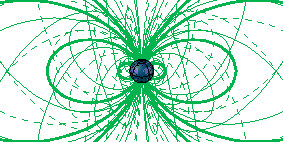
\includegraphics[scale = 1]{figure3_6a.pdf}
  	} 
 	\subfigure[]{
	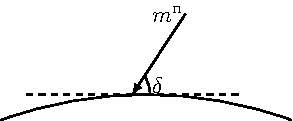
\includegraphics[scale = 1]{figure3_6b.pdf}
	} 
  \caption[]{(a) Schematic of the earth magnetic field lines (green) around the earth (blue).\footnotemark~(b) Schematic of a part of the earth where the local earth magnetic field $m^{\text{n}}$ makes an angle $\delta$ with the horizontal plane. This angle is called the dip angle.} 
  \label{fig:models-magneticField}
\end{figure}
\footnotetext{Adapted version of `Dipolar magnetic field'  by Cyril Langlois available at \url{http://texample.net} under CC BY 2.5 (\url{http://creativecommons.org/licenses/by/2.5}).}
}

In practice, the actual magnetic field can differ significantly from the earth magnetic field. In indoor environments, for instance, presence of magnetic material in the structure of buildings and in furniture influences the magnetic field that is measured by the magnetometer. Furthermore, the magnetic field is affected in applications where the magnetometer is mounted in \eg a vehicle, train or on a robot. In case the magnetic material is rigidly attached to the sensor, the magnetometer can be calibrated for its presence \citep{kokS:2016,vasconcelosESOC:2011,renaudinAL:2010,salehiMB:2012}. The presence of magnetic material in the vicinity of the sensor that can not be calibrated for is of major concern for practical applications. Because of this, there is a vast amount of literature on the topic, see \eg \cite{callmer:2013,ligorioS:2016,roetenbergLBV:2005}. 

Note that when using magnetometers for orientation estimation, the presence of magnetic material is typically considered to be an undesired disturbance. However, the presence of magnetic material can also be considered to be a property which can be exploited. This is done in approaches which use the magnetic field as a source of position information \citep{solinKWSS:2015,haverinenK:2009,robertsonFADJPKLB:2013}.

\paragraph{Position information}
Position information can be obtained from for instance \gls{gnss} or \gls{uwb} measurements. In this tutorial, we will consider a very basic measurement model where the sensors directly measure the position as
\begin{align}
\label{eq:models-posMeasModel}
y_{\text{p},t} &= p_t^\text{n} + e_{\text{p},t}, 
\end{align}
with $e_{\text{p},t} \sim \mathcal{N}(0,\Sigma_\text{p})$. 

Many sensors do not measure the position directly. Their measurements can, however, be pre-processed to obtain position estimates and their corresponding covariances~\citep{gustafssonG:2005}. For example, time of arrival measurements can be pre-processed using multilateration techniques. Measurements of this type often contain a significant amount of outliers. The reason is that the signals can be delayed due to multipath or \gls{nlos} conditions. Possible solutions deal with this by doing outlier rejection, by using robust algorithms, see \eg \cite{zoubirKCM:2012}, or by modeling the noise distribution as a non-Gaussian distribution, see \eg \cite{kokHS:2015,gustafssonG:2005,nurminenAPG:2015}. We will discuss an example of this in more detail in~\Sectionref{sec:appl-uwb}.

\section{Choosing the state and modeling its dynamics}
\label{sec:models-stateDynamics}
The fundamental continuous-time relations that form the basis of our dynamic models are the fact that the position $p^\text{n}$, velocity $v^\text{n}_\text{n}$ and acceleration $a^\text{n}_\text{nn}$ are related as 
\begin{align}
v^\text{n}_\text{n} = \left. \tfrac{\tdiff p^\text{n}}{\tdiff t} \right|_\text{n}, \qquad
a^\text{n}_\text{nn} = \left. \tfrac{\tdiff v^\text{n}}{\tdiff t} \right|_\text{n},
\label{eq:models-contTimePosVel}
\end{align}
and that the orientation and angular velocity $\omega_{\text{nb},t}^\text{b}$ are related as
\begin{align}
\tfrac{\tdiff q^\text{nb}}{\tdiff t} = q^\text{nb} \odot \tfrac{1}{2}\bar{\omega}_{\text{nb}}^\text{b}, \qquad
\tfrac{\tdiff R^\text{nb}}{\tdiff t} = R^\text{nb} [\omega_{\text{nb}}^\text{b} \times],
\label{eq:models-contTimeOri}
\end{align}
depending on orientation parametrization. For a derivation of~\eqref{eq:models-contTimeOri}, see \eg \cite{hol:2011}. Using an Euler discretization of~\eqref{eq:models-contTimePosVel} assuming that the acceleration is constant between samples, the dynamics of the position and velocity can be expressed in terms of the acceleration as
\begin{subequations}
\label{eq:models-dynModelPosVel}
\begin{align}
p^\text{n}_{t+1} &=  p_t^\text{n} + T v_{\text{n},t}^\text{n} + \tfrac{T^2}{2} a^\text{n}_{\text{nn},t}, \\
v^\text{n}_{\text{n},t+1} &= v_{\text{n},t}^\text{n} + T a_{\text{nn},t}^\text{n}, 
\end{align}
\end{subequations}
where $T$ is the time between two samples. Similarly, the dynamics of the orientation can be expressed in terms of unit quaternions or rotation matrices as
\begin{subequations}
\label{eq:models-dynModelOri}
\begin{align}
q^\text{nb}_{t+1} &= q_t^\text{nb} \odot \expq \left( \tfrac{T}{2} \omega^\text{b}_{\text{nb},t} \right), \\
R^\text{nb}_{t+1} &= R_t^\text{nb} \expR \left( T \omega^\text{b}_{\text{nb},t} \right).
\end{align}
\end{subequations}

Dynamic models describe how the state changes over time. For the problem of position and orientation estimation using inertial sensors, there are two commonly used modeling alternatives for the dynamics~\citep{gustafsson:2012}. In the first, the state vector $x_t$ is chosen to consists of  
\begin{align}
x_t = \begin{pmatrix} \left(p^\text{n}_t \right)^\Transp & \left(v^\text{n}_{\text{n},t} \right)^\Transp & \left(a^\text{n}_{\text{nn,t}} \right)^\Transp & \left(q^\text{nb}_t \right)^\Transp & \left(\omega^\text{b}_{\text{nb},t} \right)^\Transp \end{pmatrix}^\Transp.
\end{align}
The change in position, velocity and orientation states can then be described in terms of the velocity, acceleration and angular velocity states, respectively. The dynamics of the acceleration and the angular velocity can be described in terms of a \emph{motion model}. Examples of motion models that can be used are a constant acceleration model, which assumes that the dynamics of the acceleration can be described as 
\begin{align}
\label{eq:models-constAcc}
a^\text{n}_{\text{nn},t+1} = a^\text{n}_{\text{nn},t} + w_{\text{a},t},
\end{align}
with $w_{\text{a},t} \sim \mathcal{N}(0,\Sigma_\text{w,a} )$, and a constant angular velocity model, which describes the dynamics of the angular velocity as
\begin{align}
\label{eq:models-constAngVel}
\omega^\text{b}_{\text{nb},t+1} = \omega^\text{b}_{\text{nb},t} + w_{\omega,t},
\end{align}
with $w_{\omega,t} \sim \mathcal{N}(0,\Sigma_{\text{w},\omega})$. The process noise terms $w_{\text{a},t}$ and $w_{\omega,t}$ model the assumptions on how constant the acceleration and angular velocity actually are. 

Alternatively, the state vector $x_t$ can be chosen as 
\begin{align}
x_t = \begin{pmatrix} \left(p^\text{n}_t \right)^\Transp & \left(v^\text{n}_{\text{n},t} \right)^\Transp & \left(q^\text{nb}_t \right)^\Transp \end{pmatrix}^\Transp.
\end{align}
To describe the dynamics of the states, the inertial measurements can then be used as an \emph{input} to the dynamic equation~\eqref{eq:models-dynamics}. Hence, the change in position, velocity and orientation is directly modeled in terms of the inertial measurements. In this case, expressions for $a^\text{n}_{\text{nn},t}$ and $\omega^\text{b}_{\text{nb},t}$ in~\eqref{eq:models-dynModelPosVel} and~\eqref{eq:models-dynModelOri} are obtained from the accelerometer measurement model and the gyroscope measurement model, see \Sectionref{sec:models-measModels}. The process noise can explicitly be modeled in terms of the accelerometer measurement noise $e_{\text{a},t}$ and the gyroscope measurement noise $e_{\omega,t}$. 

The benefit of using a motion model for the state dynamics is that knowledge about the motion of the sensor can be included in this model. However, it comes at the expense of having a larger state vector. The benefit of using the inertial measurements as an input to the dynamics is that the process noise has the intuitive interpretation of representing the inertial measurement noise. Hence, the latter approach is often used for applications where it is difficult to obtain sensible motion models. Another difference between the two approaches is that changes in the acceleration and angular velocity will have a slightly faster effect on the state when the inertial measurements are used as an input to the dynamics. The reason for this is that the constant acceleration and angular velocity models delay the effects of changes in the dynamics. Because of this, their estimates typically look slightly more smooth. 

\section{Models for the prior}
\label{sec:models-prior}
Looking back at \Sectionref{sec:models-probModeling}, to solve the smoothing and filtering problems~\eqref{eq:models-smoothingProbs} and~\eqref{eq:models-filteringProbs}, we have now discussed different models for the dynamics $p(x_t \mid x_{t-1},\theta)$ in \Sectionref{sec:models-stateDynamics} and for the measurements $p(y_t \mid x_{t},\theta)$ in \Sectionref{sec:models-measModels}. The remaining distributions to be defined are $p(x_1 \mid \theta)$ and $p(\theta)$. Note that we typically assume that $x_1$ is independent of $\theta$. Hence, in this section we focus on the prior distributions $p(x_1)$ and $p(\theta)$.

In many cases, there is fairly little prior information available about the parameters $\theta$. It is, however, often possible to indicate reasonable values for the parameters. For example, it is reasonable to assume that the gyroscope bias is fairly small but can be both positive and negative. For instance, for the data presented in \Exampleref{ex:sensors-inertialMeasurements}, the average bias over the 55-minute data set was $\begin{pmatrix} 35.67 & 54.13 & -1.07 \end{pmatrix}^\Transp \cdot 10^{-4}~\radianpersecond$. If we would assume that in $68\%$ of the cases, the bias is within the bounds $-\sigma_{\delta_\omega} \leq \delta_{\omega,t}^\text{b} \leq \sigma_{\delta_\omega}$ with $\sigma_{\delta_\omega} = 5 \cdot 10^{-3}$, a reasonable prior would be
\begin{align}
\delta_{\omega,t}^\text{b} \sim \mathcal{N}(0,\sigma^2_{\delta_\omega} \mathcal{I}_3).
\end{align}

For the prior $p(x_1)$, it is typically possible to get a reasonable estimate from data. For the position and velocity, this can be modeled as
\begin{subequations}
\begin{align}
p^\text{n}_1 &= \initEst{p}_1^\text{n} + e_{\text{p,i}}, \quad & e_{\text{p,i}} &\sim \mathcal{N}(0, \sigma^2_{\text{p,i}} \mathcal{I}_3), \\
v^\text{n}_1 &= \initEst{v}_1^\text{n} + e_{\text{v,i}}, \quad & e_{\text{v,i}} &\sim \mathcal{N}(0, \sigma^2_{\text{v,i}} \mathcal{I}_3).
\end{align}
\end{subequations}
Here, the estimate $\initEst{p}_1^\text{n}$ can for instance be determined based on the first position measurement. In that case, the uncertainty $\sigma_{\text{p,i}}$ can also be chosen equal to the uncertainty of the position measurements. In case no additional information is available, the estimates $\initEst{p}_1^\text{n}$ and $\initEst{v}_1^\text{n}$ can be set to zero with an appropriate standard deviation instead.

A commonly used method to determine the initial orientation is to use the first accelerometer and magnetometer samples. This method is based on the fact that given two (or more) linearly independent vectors in two coordinate frames, the rotation between the two coordinate frames can be determined. The implicit assumption is that the accelerometer only measures the gravity vector and the magnetometer only measures the local magnetic field. Hence, the four vectors are given by the measurements $y_{\text{a},t}$ and $y_{\text{m},t}$, the local gravity vector $g^\text{n}$ and the local magnetic field $m^\text{n}$. These vectors are linearly independent except when the measurements are obtained on the magnetic north or south poles where the dip angle is $\delta = 0$ and the magnetic field does not contain any heading information. 

The accelerometer provides information about the sensor's inclination. Heading information is provided by the magnetometer. However, at all locations except on the equator, the magnetometer also provides information about the inclination due to its non-zero vertical component, see \eqref{eq:models-localMagField}. In practice, the accelerometer typically provides more accurate inclination information. Hence, we choose to use the magnetometer only to provide heading information by projecting the magnetic field and the magnetometer measurement on the horizontal plane. Furthermore, we normalize the vectors. Because of this, an adapted model uses the four normalized vectors
\begin{subequations}
\label{eq:models-oriAccMagVectors}
\begin{align}
\hat{g}^\text{n} &= \begin{pmatrix} 0 & 0 & 1 \end{pmatrix}^\Transp,  \qquad
\hat{g}^\text{b} = \tfrac{y_{\text{a},1}}{\| y_{\text{a},1} \|_2}, \\
\hat{m}^\text{n} &= \begin{pmatrix} 1 & 0 & 0 \end{pmatrix}^\Transp, \qquad 
\hat{m}^\text{b} = \hat{g}^\text{b} \times \left( \tfrac{y_{\text{m},1}}{\| y_{\text{m},1} \|_2}  \times \hat{g}^\text{b}\right).
\end{align}
\end{subequations}
A number of algorithms are available to estimate the orientation from these vectors. Well-known examples are the TRIAD algorithm, the QUEST algorithm, see \eg \cite{shusterO:1981}, and the method presented in~\cite{horn:1987}. For our problem at hand, these methods give equivalent results, even though they use slightly different solution strategies. Generally speaking, they solve the problem of determining the rotation $q^\text{nb}$ from 
\begin{align}
\label{eq:models-oriAccMag}
&\argmin_{q^\text{nb}} &&\| \bar{\hat{g}}^\text{n} - q^\text{nb} \odot \bar{\hat{g}}^\text{b} \odot q^\text{bn} \|^2_2 +  
\| \bar{\hat{m}}^\text{n} - q^\text{nb} \odot \bar{\hat{m}}^\text{b} \odot q^\text{bn} \|^2_2 \nonumber \\
& \st &&\| q^\text{nb} \|_2 = 1,
\end{align}
Recall from~\eqref{eq:models-rotatex_q} that $q^\text{nb} \odot \bar{x}^\text{b} \odot q^\text{bn}$ is the rotation of the vector $x^\text{b}$ to the $n$-frame. The optimization problem~\eqref{eq:models-oriAccMag} therefore determines the orientation $q^\text{nb}$ that minimizes the distance between the normalized magnetic field and gravity vectors measured in the first sample and the normalized magnetic field and gravity vectors in the navigation frame. These four vectors were defined in~\eqref{eq:models-oriAccMagVectors}.

Defining 
\begin{align}
A = - \left( \bar{\hat{g}}^\text{n} \right)^\leftMult \left( \bar{\hat{g}}^\text{b} \right)^\rightMult - \left( \bar{\hat{m}}^\text{n} \right)^\leftMult \left( \bar{\hat{m}}^\text{b} \right)^\rightMult,
\end{align}
where the left and right quaternion multiplications are defined in~\eqref{eq:models-leftRightQuatMult}, \eqref{eq:models-oriAccMag} can equivalently be written as 
\begin{align}
\initEst{q}^\text{nb}_1 = &\argmin_{q^\text{nb}} \quad \left( q^\text{nb} \right)^\Transp A q^\text{nb} \nonumber \\
&\st \quad \| q^\text{nb} \|_2 = 1.
\label{eq:models-oriAccMagReform}
\end{align}
For a derivation, see \cite{hol:2011}. The solution to this problem is given by the eigenvector corresponding to the largest eigenvalue of $A$. Note that although this method can be used to compute the orientation from any two linearly independent vectors in two coordinate frames, we only use it to compute a prior on the orientation. 

Based on the estimate $\initEst{q}_1^\text{nb}$ from~\eqref{eq:models-oriAccMagReform}, we can model the orientation at time $t = 1$ in terms of an orientation deviation
\begin{subequations}
\begin{align}
q_1^\text{nb} &= \expq \left( \tfrac{e_{\oriError,\text{i}}}{2} \right) \odot \initEst{q}_1^\text{nb},  & e_{\oriError,\text{i}} &\sim \mathcal{N}(0, \Sigma_{\oriError,\text{i}}), \\
\intertext{or in terms of a quaternion as}
q_1^\text{nb} &= \initEst{q}_1^\text{nb} + e_\text{q,i},  & e_\text{q,i} &\sim \mathcal{N}(0, \Sigma_\text{q,i}) .
\end{align}
\end{subequations}
Explicit formulations for the covariance of the orientation estimates from the TRIAD and QUEST algorithms are discussed by \cite{shuster:2006}. In practice, however, the accuracy of the estimates from~\eqref{eq:models-oriAccMagReform} highly depends on the validity of the model assumptions, \ie on whether the sensor is indeed far from magnetic material and whether the linear acceleration is indeed zero. Because this has such a significant influence on the quality of the estimates, we choose $\Sigma_{\oriError,\text{i}}$ and $\Sigma_\text{q,i}$ somewhat conservatively. Modeling that in $68 \%$ of the cases the orientation error is less than $20^\circ$, 
\begin{subequations}
\begin{align}
\Sigma_{\oriError,\text{i}} &= \sigma_{\oriError, \text{i}}^2 \mathcal{I}_3, \qquad \qquad \sigma_{\oriError,\text{i}} = \tfrac{20}{180} \pi, \\
\Sigma_{\text{q,i}} &= \tfrac{1}{4} \left( \initEst{q}_1^\text{nb} \right)^\rightMult \tfrac{\diff \expq (e_{\oriError,\text{i}})}{\diff e_{\oriError,\text{i}}} \Sigma_{\oriError,\text{i}} \left( \tfrac{\diff \expq (e_{\oriError,\text{i}})}{\diff e_{\oriError,\text{i}}} \right)^\Transp \left( \initEst{q}_1^\text{bn} \right)^\rightMult,
\end{align}
\end{subequations}
where we use the fact that $( q^\rightMult )^\Transp = (q^\conj)^\rightMult$. Note that the covariance $\Sigma_{\text{q,i}}$ is defined in terms of the covariance $\Sigma_{\oriError,\text{i}}$ to allow for explicit comparison between different algorithms in \Chapterref{cha:orientationEstimation}.

\section{Resulting probabilistic models}
\label{sec:models-resultingProbModel}
The information from the previous sections can now be combined into one model which will be used in the algorithms in \Chapterref{cha:orientationEstimation}. In this section, we describe our modeling choices for the pose estimation problem and for the orientation estimation problem. 

We assume that the sensor does not travel over significant distances as compared to the size of the earth and hence keep the navigation frame $n$ fixed with respect to the earth frame $e$. Furthermore, we assume that the magnitude of the earth rotation and of the Coriolis acceleration are negligible. Our gyroscope and accelerometer models are hence given by 
\begin{subequations}
\begin{align}
y_{\text{a},t} &= R^{\text{bn}}_t  ( a_{\text{nn}}^\text{n} - g^\text{n} ) + \delta_{\text{a},t}^\text{b} + e_{\text{a},t}^\text{b}, \label{eq:models-accMeasModelRes} \\
y_{\omega,t} &= \omega_{\text{nb},t}^\text{b} + \delta_{\omega,t}^\text{b} + e_{\omega,t}^\text{b}. \label{eq:models-gyrMeasModelRes}
\end{align}
\end{subequations}
In the remainder, for notational convenience we drop the subscripts $n$ which indicate in which frame the differentiation is performed, see \Sectionref{sec:sensors-specForce}, and use the shorthand notation $a^\text{n}$ for $a_{\text{nn}}^\text{n}$. Furthermore, we will denote $\omega_{\text{nb}}^\text{b}$ simply by $\omega$ and omit the superscript $b$ on the noise terms $e_{\text{a},t}$ and $e_{\omega,t}$ and the bias terms $\delta_{\text{a},t}$ and $\delta_{\omega,t}$. We assume that the inertial measurement noise is given by
\begin{align}
e_{\text{a},t} \sim \mathcal{N}(0, \sigma_\text{a}^2 \, \mathcal{I}_3 ), \qquad e_{\omega,t} \sim \mathcal{N}(0, \sigma_\omega^2 \, \mathcal{I}_3 ),
\label{eq:models-assumptionNoiseDiag}
\end{align}
\ie we assume that the three sensor axes are independent and have the same noise levels. 

\subsection{Pose estimation}
For pose estimation, we model the accelerometer and gyroscope measurements as inputs to the dynamics. Hence, the state vector consists of the position $p^\text{n}_{t}$, the velocity $v^\text{n}_{t}$ and a parametrization of the orientation. We use the inertial measurements in combination with position measurements to estimate the pose. 

Using the accelerometer measurement model \eqref{eq:models-accMeasModelRes} in~\eqref{eq:models-dynModelPosVel}, the dynamics of the position and velocity is given by 
\begin{subequations}
\begin{align}
p_{t+1}^\text{n} &= p_t^\text{n} + T v_t^\text{n} + \tfrac{T^2}{2} \left( R^\text{nb}_t (y_{\text{a},t} - \delta_{\text{a},t}) + g^\text{n} + e_{\text{a},t} \right), \\
v_{t+1}^\text{n} &= v_t^\text{n} + T \left( R^\text{nb}_t (y_{\text{a},t} - \delta_{\text{a},t}) + g^\text{n} + e_{\text{a},t} \right),
\end{align}
\end{subequations}
where without loss of generality, we switch the sign on the noise. Note that the noise term $e_{\text{a},t}$ should be rotated to the navigation frame $n$ by multiplying it with the rotation matrix $R^\text{nb}_t$. However, because of the assumption~\eqref{eq:models-assumptionNoiseDiag}, the rotation matrix can be omitted without loss of generality. The dynamics of the orientation parametrized using quaternions is given by
\begin{align}
q^\text{nb}_{t+1} &= q_t^\text{nb} \odot \expq \left( \tfrac{T}{2} (y_{\omega,t} - \delta_{\omega,t} - e_{\omega,t} ) \right).
\end{align}
Equivalent dynamic models can be obtained for the other parametrizations. 

The position measurements are modeled as in~\eqref{eq:models-posMeasModel}. In summary, this leads to the following state space model for pose estimation
\begin{subequations}
\label{eq:models-ssPose}
\begin{align}
\begin{pmatrix} 
p^\text{n}_{t+1} \\
v^\text{n}_{t+1} \\ 
q^\text{nb}_{t+1} 
\end{pmatrix}
&= \begin{pmatrix} 
p_t^\text{n} + T v_t^\text{n} + \tfrac{T^2}{2} \left( R^\text{nb}_t (y_{\text{a},t} - \delta_{\text{a},t}) + g^\text{n} + e_{\text{p,a},t} \right) \\
v_t^\text{n} + T \left( R^\text{nb}_t (y_{\text{a},t}  - \delta_{\text{a},t}) + g^\text{n} + e_{\text{v,a},t} \right) \\
q_t^\text{nb} \odot \expq \left( \tfrac{T}{2} (y_{\omega,t} - \delta_{\omega,t} - e_{\omega,t} ) \right)
\end{pmatrix}, \label{eq:models-ssPose-dyn} \\
y_{\text{p},t} &= p_t^\text{n} + e_{\text{p},t}, \label{eq:models-ssPose-meas}
\intertext{where}
e_{\text{p,a},t} &\sim {\mathrlap{\mathcal{N}(0, \Sigma_\text{a} ),}\phantom{\bar{q}_1^\text{nb} \odot \expq ( \tfrac{e_{\oriError,\text{i}}}{2} )}} \qquad \, e_{\text{v,a},t} \sim \mathcal{N}(0, \Sigma_\text{a} ), \\
e_{\text{p},t} &\sim {\mathrlap{\mathcal{N}(0, \Sigma_\text{p} ),}\phantom{\bar{q}_1^\text{nb} \odot \expq ( \tfrac{e_{\oriError,\text{i}}}{2} ), \, \qquad}} \, e_{\omega,t} \sim \mathcal{N}(0, \Sigma_\omega ), 
\intertext{with $\Sigma_\text{a} = \sigma_\text{a}^2 \, \mathcal{I}_3$ and $\Sigma_\omega = \sigma_\omega^2 \, \mathcal{I}_3$. Note that we model the process noise on the position and velocity states in terms of the accelerometer noise. However, we do not enforce these to have the same noise realization. Hence, we use the notation $e_{\text{p,a},t}$ and $e_{\text{v,a},t}$ for the two process noise terms. The covariance of both is equal to the covariance of the accelerometer noise. The initial position is assumed to be given by the first position measurement as}
p^\text{n}_1 &= {\mathrlap{y_{\text{p},1} + e_{\text{p,1}},}\phantom{\bar{q}_1^\text{nb} \odot \expq ( \tfrac{e_{\oriError,\text{i}}}{2} ),}} \, \qquad \, e_{\text{p,1}} \sim \mathcal{N}(0, \Sigma_\text{p,i}), 
\intertext{while the initial velocity is assumed to be approximately zero as}
v^\text{n}_1 &= {\mathrlap{e_{\text{v,i}},}\phantom{\bar{q}_1^\text{nb} \odot \expq ( \tfrac{e_{\oriError,\text{i}}}{2} ),}} \, \qquad \, \, e_{\text{v,i}} \sim \mathcal{N}(0, \Sigma_{\text{v,i}}).
\intertext{The orientation at time $t = 1$ is given by the QUEST algorithm described in \Sectionref{sec:models-prior}, parametrized in terms of quaternions or rotation vectors as }
q_1^\text{nb} &= \expq \left( \tfrac{e_{\oriError,\text{i}}}{2} \right) \odot \initEst{q}_1^\text{nb}, \qquad e_{\oriError,\text{i}} \sim \mathcal{N}(0, \Sigma_{\oriError,\text{i}}), \label{eq:models-ssPose-priorOriDev} \\
q_1^\text{nb} &= { \mathrlap{\initEst{q}_1^\text{nb} + e_\text{q,i},}\phantom{\bar{q}_1^\text{nb} \odot \expq ( \tfrac{e_{\oriError,\text{i}}}{2} ),} } \qquad \, \, e_\text{q,i} \sim \mathcal{N}(0, \Sigma_\text{q,i}), \label{eq:models-ssPose-priorQuat}
\end{align}
\end{subequations}
where the initial orientation uncertainty is given in terms of a standard deviation of $20^\circ$.

In \Chapterref{cha:orientationEstimation} we assume that the inertial measurement are properly calibrated. Hence, we assume that their biases $\delta_{\text{a},t}$ and $\delta_{\omega,t}$ are zero. Calibration is the topic of \Chapterref{cha:calibration} where we will also introduce possible extensions of the state space model in which the bias terms are included either as states or as unknown parameters.

\subsection{Orientation estimation}
For orientation estimation, the state vector only consists of a parametrization of the orientation. We use the inertial sensors in combination with the magnetometer measurements to estimate the orientation. The magnetometer measurements are modeled as in~\eqref{eq:models-magMeasModel}. Instead of using the accelerometer measurements model~\eqref{eq:models-accMeasModelRes}, we use the model~\eqref{eq:models-accMeasModelZeroAcc} where it is assumed that the linear acceleration is approximately zero. This leads to the following state space model for orientation estimation,
\begin{subequations}
\label{eq:models-ssOri}
\begin{align}
q^\text{nb}_{t+1} &= q_t^\text{nb} \odot \expq \left( \tfrac{T}{2} (y_{\omega,t} - \delta_{\omega} - e_{\omega,t} ) \right), \label{eq:models-ssOri-dyn} \\
y_{\text{a},t} &= - R^\text{bn}_t g^\text{n} + e_{\text{a},t} , \label{eq:models-ssOri-measAcc} \\
y_{\text{m},t} &= R^\text{bn}_t m^\text{n} + e_{\text{m},t}, \label{eq:models-ssOri-measMag}
\intertext{where~\eqref{eq:models-ssOri-dyn} describes the dynamics while~\eqref{eq:models-ssOri-measAcc} and~\eqref{eq:models-ssOri-measMag} describe the measurement models and} 
e_{\omega,t} &\sim \mathcal{N}(0,\Sigma_\omega), \qquad e_{\text{a},t} \sim \mathcal{N}(0, \Sigma_\text{a}), \qquad e_{\text{m},t} \sim \mathcal{N}(0,\Sigma_\text{m}),
\end{align}
\end{subequations}
with $\Sigma_\omega = \sigma_\omega^2 \, \mathcal{I}_3$ and $\Sigma_\text{a} = \sigma_\text{a}^2 \, \mathcal{I}_3$. The initial orientation is given by the QUEST algorithm described in \Sectionref{sec:models-prior} and is modeled as in~\eqref{eq:models-ssPose-priorOriDev} or~\eqref{eq:models-ssPose-priorQuat}. Also for orientation estimation, in \Chapterref{cha:orientationEstimation} we assume that the inertial measurements are properly calibrated. Hence, we assume that the bias $\delta_{\omega,t}$ is zero.